% INFORMATION
\def\projectinfoleft{
  Author: \\
  Project Supervisor: \\
  Project Assessor:
}
\def\projectinforight{
  Juntong Liu (201219267) \\
  Dr Mark Bowden \\
  Dr James Walsh
}
\def\studentname{
  \includegraphics[width=0.15\textwidth,
  bb=-200 200 1936 650]{signature}}
\def\reporttitle{
  \bf Final Report for Project: \\Development of a C++ User-interface\\ for a Plasma Simulation Tool}
\def\theabstract{ %
In this project, a program is developed to view data generated in plasma simulations with options to export the data into images and videos, then further expanded to be a general purposed data viewing tool. The development uses C++ as the main language, with a plugin system implemented in Python. The implementation of user interface uses Qt as framework, and provides diagram rendering in 2D and 3D space using OpenGL. This article describes the design of the project, then focuses on the implementation of the framework, including test results of libraries used in this project. Afterwards, overview of the program is given and output files is compared to files generated by other programs. Finally, suggestions for future improvements are given for reference.
}
% INFORMATION END

\documentclass[12pt, a4paper]{article}
\usepackage{graphicx, fullpage, listings}
\usepackage{pdfpages, color}
\usepackage[titletoc, page]{appendix}
\usepackage{tocloft}
\usepackage{ifthen, calc}
\usepackage{subfig, wrapfig, caption}
\usepackage{lipsum}
\usepackage[separate-uncertainty=true, multi-part-units=single, output-complex-root = j, complex-root-position = before-number]{siunitx}
\usepackage{amsmath}
\usepackage[hyphens]{url}
\usepackage[siunitx, american]{circuitikz}
\usepackage[hidelinks]{hyperref}
\usepackage{cprotect}
\usepackage{suffix}
\usepackage{enumitem}
\usepackage[hang,flushmargin]{footmisc}
\usepackage{lmodern}
\usepackage{float}

% COMMANDS

\newfloat{lstfloat}{tbp}{lop}
\floatname{lstfloat}{Listing}
\def\lstfloatautorefname{Listing}

\newcommand\cell[2]{\parbox{#1\textwidth}{\vspace{3pt}#2\vspace{3pt}}}

\newcommand\makereference[1]{ %
  \bibliographystyle{res/myieee}
  \bibliography{#1}
  \addcontentsline{toc}{section}{References}
}

% \eq[label]{equation}
\newcommand\eq[2][]{ %
  \ifthenelse{\equal{#1}{}}{ %
    \begin{equation*}\begin{aligned} #2 \end{aligned}\end{equation*}
  }{ %
    \begin{equation}\begin{aligned} #2 \end{aligned}\label{#1}\end{equation}
  }
}

\newcommand{\MatLab}{\textsc{Matlab}}

% VALUES
\graphicspath{{fig/}}
\setlength\cftbeforesecskip{3pt}
\setlength{\parskip}{4.5pt}
\interfootnotelinepenalty=500
\hfuzz=\maxdimen
\tolerance=10000
\hbadness=10000
\setlist[itemize]{topsep=0.5pt}


% LISTING

\lstdefinelanguage{ahdl}{
  morekeywords={
    AND, ASSERT, BEGIN, BIDIR, BiTS, BURIED,
    CASE, CLIQUE, CONNECTED_PINS, CONSTANT,
    DEFAULTS, DEFINE, DESIGN, DEVICE, DIV,
    ELSE, ELSEIF, END, FOR, FUNCTION,
    GENERATE, GND, HELP_ID,
    IF, INCLUDE, INPUT, IS, LOG2,
    MACHINE, MOD, NAND, NODE, NOR, NOT,
    OF, OPTIONS, OR, OTHERS, OUTPUT,
    PARAMETERS, REPORT, RETURNS,
    SEGMENTS, SEVERITY, STATES, SUBDESIGN,
    TABLE, THEN, TITLE, TO, TRI_STATE_NODE,
    VARIABLE, VCC, WHEN, WITH, XNOR, XOR,
    CARRY, CASCADE, CEIL, DFFE, DFF,
    EXP, FLOOR, GLOBAL, JEFFE, JKFF,
    LATCH, LCELL, MCELL, MEMORY, OPNDRN,
    SOFT, SRFFE, SRFF, TFFE, TFF, TRI,
    WIRE, X
  },
  sensitive=false,
  morecomment=[l]{--},
  morecomment=[s]{\%}{\%},
  tabsize = 4
}

\lstdefinelanguage{xml}{
  basicstyle=\ttfamily\footnotesize,
  morestring=[b]",
  moredelim=[s][\bfseries\color{mygreen}]{<}{\ },
  moredelim=[s][\bfseries\color{mygreen}]{</}{>},
  moredelim=[l][\bfseries\color{mygreen}]{/>},
  moredelim=[l][\bfseries\color{mygreen}]{>},
  morecomment=[s]{<?}{?>},
  morecomment=[s]{<!--}{-->},
  commentstyle=\color{mygrey},
  stringstyle=\color{myorange},
  %identifierstyle=\color{mygreen}
}

\newcommand\lstinputlistingnobreak[2][]{
  \begin{figure}[!ht]
  \vspace{-0.5cm}
  \lstinputlisting[#1]{#2}
  \end{figure}
}

\lstnewenvironment{lstlistingnobreak}[1][]{ %
  \figure[!ht]\vspace{-0.5cm}
  \lstset{xrightmargin=35pt}\lstset{#1}
}{ %
  \endfigure
}

\lstset{
  frame=single,basicstyle=\ttfamily,breaklines=true
}

\definecolor{myyellow}{rgb}{1,1,0.8}
\definecolor{mygray}{rgb}{0.5,0.5,0.4}
\definecolor{mygreen}{rgb}{0,0.7,0.5}
\definecolor{myorange}{rgb}{1.0,0.4,0}
\definecolor{mylilas}{rgb}{0.8,0.3,1.0}

\lstdefinestyle{mybase} {
	breaklines=true,
	showstringspaces=false,
	basicstyle=\scriptsize\tt,
	frame=single,
	xleftmargin=20pt,
	xrightmargin=20pt,
  numbersep=9pt,
  numberstyle={\color{black} \footnotesize \sf},
  stringstyle=\color{myorange},
  keywordstyle=\color{mygreen},
  commentstyle=\color{mygray},
  tabsize=4
}

\lstdefinestyle{myahdl} {
  style=mybase,
  language = ahdl,
  keywordstyle=\color{mylilas},
  commentstyle=\color{mygreen}
}

\lstdefinestyle{mymatlabcode} {
  style=mybase,
	language=Matlab,
	stringstyle=\color{mylilas},
	commentstyle=\color{mygreen},
	emph=[1]{for,end,break,function,while,if,else},emphstyle=[1]\color{blue},
}

\lstdefinestyle{mymatlabconsole} {
  style=mybase,
	morecomment=[l][\color{red}]{Error},
}

\lstdefinestyle{myahdl} {
  style=mybase,
  language = ahdl,
  keywordstyle=\color{mylilas},
  commentstyle=\color{mygreen},
  numberstyle={\color{black} \footnotesize \sf}
}


% TITLE

\title{
  \includegraphics[width=0.4\textwidth]{res/univcrest.pdf}
  \\[4pt]\reporttitle}
\author{ %
\begin{minipage}{0.4\textwidth}
\begin{flushleft}
  \projectinfoleft
\end{flushleft}
\end{minipage}
\begin{minipage}{0.4\textwidth}
\begin{flushright}
  \projectinforight
\end{flushright}
\end{minipage}
}
\date{\small{\today}}

\usepackage[super]{nth}
\usepackage{pdfpages}
\begin{document}

\begin{titlepage}
\maketitle
\thispagestyle{empty}
\addtocontents{toc}{\protect\thispagestyle{empty}}

\begin{center}
  \textbf{Declaration of academic integrity}
\end{center}
\begin{small}
  \noindent I confirm that I have read and understood the University's Academic Integrity Policy.

  \noindent I confirm that I have acted honestly, ethically and professionally in conduct leading to assessment for the programme of study.

  \noindent I confirm that I have not copied material from another source nor committed plagiarism nor fabricated, falsified or embellished data when completing the attached piece of work.

  \noindent I confirm that I have not copied material from another source, nor colluded with any other student in the preparation and production of this work.
  \begin{flushright}
  \begin{tabular}{ m{0.1\linewidth} m{0.25\linewidth}  }
    \hfuzz=5pt 
    Signature:  & \studentname  \\
    Date: & \today  \\
  \end{tabular}
  \end{flushright}

\end{small}

\begin{center} \textbf{Abstract} \end{center}
\begin{small}
\theabstract
\end{small}

\begin{center}
\begin{minipage}{\linewidth}
\tableofcontents
\end{minipage}
\end{center}
\end{titlepage}


\section{Introduction}

Simulation programs are helpful tools in plasma research. Usually they accept plasma models, then use it to generate a variety of quantities related to the model with progress of time. Plasimo is one of plasma simulation programs. It is powerful in simulation, but is not so convenient to view the generated data. As given in figure \ref{fig:plasimo}, it provides rendering of the quantities, but only for the current state of the model. However, some models might take hours or even days to simulate, it will become troublesome if the user wants to view the data generated in previous time. For the previous data, Plasimo will write them into text files, which are usually with big file size for long-time simulations, making it difficult for a human to read. In addition, if the user wants to render the data in tools like \MatLab{} or Excel, the user also needs to find the specific data section and convert the it to some format that is acceptable to the rendering programs, which also increases the inconvenience.

\begin{figure}[!htb]
	\centering
	\includegraphics[width=0.7\textwidth]{plasimo}
	\caption{Screenshot of Plasimo interface\cite{ref:plasimo}}
	\label{fig:plasimo}
\end{figure}

The primary object of this project is to develop a program to handle these output files, then convert them into a format that is more user-friendly, the typical way of which is analyse the files, then render them as diagrams with a graphical user interface. In addition, to make a complete workflow, the program should be able to export the data into other formats. Although he focused data format of this project is MD2D format generated by Plasimo, the applications might be limited if this project only supports data in this format. Therefore, it could be better to handle user-defined data formats, to make it as a universal data processing tool for different data formats.

\section{Background}

\subsection{Industrial Relevance}

\begin{figure}[!tb]
	\centering
	\includegraphics[width=0.7\textwidth]{echarts}
	\caption{Demonstration of ECharts}
	\label{fig:echarts}
\end{figure}


Data visualization is a hot topic in industry, and projects like ECharts\cite{ref:echarts} and Data Studio\cite{ref:datastudio} is getting attention. However, recent development of data visualization tools mainly focuses on being interactive, attractive, creative and web based. On the other side, the market of traditional data rendering tools is mainly occupied by professional software packages like \MatLab{}, SPSS and Excel, in which data rendering is provided as one of the features included in the package. Compared to the projects mentioned, this project has following characteristics:
%
\begin{itemize}
	\item This project is free and open source, making it accessible to normal users. For experienced developers, they can even modify the code to implement their required features, then redistribute it, which is impossible to most of commercial projects.
	\item The project is dedicated to data rendering and the main program is natively written in C++ with rendering implemented in OpenGL, the combination of which could provide top-level performance in mainstream software development, enabling it for real-time data rendering even with large data samples in 3D space.
	\item The program is light-weighted. For the released binary file, it takes less than \SI{17}{MB} on Windows, and less than \SI{1}{MB} on Linux. So the program can be easily copied to flash disks or shared through Internet. In addition, the plugins are script files with no dependencies, no requirement for compilation and no difference on all platforms.
	\item Compared to web-based data visualizing products, the style is suitable for academic use.
\end{itemize}


Generally speaking, this project focuses on a specific scenario of data visualization, but it has descent performance for large groups of data, reasonable rendering quality, zero-configuration experience and most importantly, flexibility for customization.

This project can also be a good reference to programmers developing OpenGL rendering, Qt--OpenGL integration or Python--C++ integration, which are all widely required features but with difficulty in development. The size of this project is not suitable as a minimum example, but it provides typical and cross-platform implementation of topics mentioned, with reasonable performance, making it a good example for practical development.

\subsection{Similar Projects}

\subsubsection{Comparison with \MatLab{}}

As a widely used industrial standard mathematical tool, \MatLab{} (and its open source alternate Octave \cite{ref:octave}) provides powerful functionalities for data rendering. Users are given many options to adjust nearly every aspect related to appearance of diagrams. Figure \ref{fig:matlab0} shows a basic example generated by \MatLab{}.

\begin{figure}[tb]
	\centering
	\subfloat[Function $y = e^x$]{
		\includegraphics[width=0.48\textwidth]{matlab0}
		\label{fig:matlab0}
	} \\
	\subfloat[Small grid 1]{
		\includegraphics[width=0.48\textwidth]{matlab1}
		\label{fig:matlab1}
	}
	\subfloat[Small grid 2]{
		\includegraphics[width=0.48\textwidth]{matlab2}
		\label{fig:matlab2}
	}
	\caption{Example outputs from \MatLab}
	\label{fig:octave}
\end{figure}

It is powerful in data rendering, but still has some disadvantages:
%
\begin{itemize}
	\item Scripts are the primary method of interaction. This could be helpful to high level users because it can be easily reused and distributed, but for starters, they might get confused easily and find it difficult to start.
	\item Although it has many options to configure, the default settings for diagrams are not good enough to be used directly in academic writing. For example, the default font size is usually too small to read when used in articles.
	\item For surface with limited data points, the rendering is not symmetrical in both colour and surface cutting. Figure \ref{fig:matlab1} and \ref{fig:matlab2} give the rendering at different angle of a $4\times4$ grid with ones in the centre surrounded by zeros, in which differences can be easily noticed. Although the difference can be ignored in large grids, space of improvement can be recognized.
	\item When rendering vector images with interpolation enabled, bitmaps are widely used to generate the gradient in the diagrams, which loses the lossless-scaling feature of vector images, and increases file size.
	\item \MatLab{} is a commercial software, which is very expensive for normal users.
\end{itemize}

\subsubsection{Comparison with Excel}

\begin{figure}[tb]
	\centering
	\subfloat[Function example]{
		\includegraphics[width=0.45\textwidth]{excel1}
		\label{fig:excel1}
	} \hspace{1em}
	\subfloat[Surface example]{
		\includegraphics[width=0.45\textwidth]{excel2}
		\label{fig:excel2}
	}
	\caption{Example outputs from Excel}
	\label{fig:excel}
\end{figure}

Excel is widely used in statistics, but plot generation is also an important feature. Figure \ref{fig:excel} shows two example figures generated by Excel. From the figures, it can be noticed the quality of the rendering is descent, even for data set with limited size (figure \ref{fig:excel2} uses the same data as figure \ref{fig:matlab1} and figure \ref{fig:matlab2}). Different from \MatLab{} and Octave, the style used by Excel is more suitable for commercial usage, although it can be suitable for academic purpose after some adjustments. The main drawback of Excel is that it only supports files in specific encoding like XLS, CSV and XML. For user-defined file encoding, it might be troublesome to supply to the program because it is designed to manipulate the data in standard data formats and user-defined data format can easily lost compatibility with some features. Therefore, to use Excel for data rendering of user-defined formats, the user usually need to use other programs or scripts to convert the data into formats supported. Another problem is Office is also a commercial product, so it can be expensive for personal users.

\subsection{Real-world Applicability}

As stated in previous sections, the primary object of this project is to develop a data viewing tool for data files generated by plasma simulation. For users using it to view simulation data, they are provided with a user interface to open and view the data. For the simulation model, the program can display multiple quantities in the same screen with a slider bar to choose the time. Compared to professional programs like \MatLab{}, it provides a more flexible and organized user-interface, making it easier to learn and use. But considering the project scale, \MatLab{} provides more options to configure the diagram style, so the user can adjust the rendering according to their tastes.

For users not using this program to view plasma models, due to the flexibility of the framework, this program supports nearly all the methods to acquire data programmatically, including serial ports and online data. In addition, although it is not currently supported, the plugin framework can be easily modified to accept data stream. Some possible applications are given as follows:

\begin{itemize}
	\item For researchers, the program can be used to render different kinds of data. Listing \ref{code:gnucap} shows an example output file generated by Gnucap (a circuit simulation software). This program can easily read and separate different quantities in the file through a plugin, then render them as functions of time.
	\item For system administrators, it can be used to monitor the state of local computer, or even remove servers through internet. The user interface can display many attributes of the system on the same screen, which could be helpful to the user.
	\item For hardware developers, the program can be used to monitor serial data. With help of plugins, the user can easily support customized protocols, even for multiple quantities with different encoding, which is not a common feature in programs at this size.
\end{itemize}

For applications listed, usually there are different programs developed for each scenario. For example, Windows System Monitor to view the state of a computer, serial plotter in Arduino IDE to plot serial data. However, with the help of plugins, this program can handle all of the scenarios. Although it will not be able to provide some specific information compared to dedicated programs, it seems to be good enough to personal users, or as an alternate if there is no dedicated programs. For the three applications listed, typically the plugin should take less than 100 lines. For the MD2D format, which is a data format containing multiple files and multiple encodings in different files, the built-in plugin for this format takes about 300 lines. In most of the cases, writing a plugin is convenient enough for experienced developers.

\begin{lstlisting}[style = mybase, caption = Example output file from Gnucap, label = code:gnucap]
#Time       v(1)       v(2)       v(3)       v(4)
0.         0.         0.         0.         0.
100.E-6    1.154E-9   0.057701   0.062791   0.11286
200.E-6    2.2955E-9  0.11477    0.12533    0.22427
300.E-6    3.4121E-9  0.1706     0.18738    0.33282
400.E-6    4.4917E-9  0.22458    0.24869    0.43712
500.E-6    5.5227E-9  0.27613    0.30902    0.53583
......
\end{lstlisting}

\subsection{Scientific Impact}

The main aim of this project is to provide a convenient tool to view the formatted data, especially generated in plasma simulation. For all the researchers having difficulty reading large samples of data, this program provides descent user experience and a clear representation of data, which could be helpful when analysing data. Compared to \MatLab{} scripts, it is easier to use and faster in response.

In addition to viewing the data, this program is also able to export the diagrams into images, or videos. These multimedia materials are usually more attractive and intuitive to students compared to data and theories. Therefore, this project could make it easier to introduce the model and the logic to others.

Compared to professional data processing products like \MatLab{} and Excel, which are usually very expensive, it is free and open source. Therefore, this project makes it accessible to everyone to the convenience of data visualization tools.

\section{Design}

\subsection{User Interaction}

This project aims to provide user-friendly experience, even for beginners. So this project will provide completely GUI based experience for daily usage, without any requirement of scripting. For plasma simulation, the result is usually difficult for people to read because the model includes many quantities and for 2D models, the output data will have the format of matrices. This matrices are usually translated to surfaces (scalar field) and vector plots (vector field), making it difficult to render one quantity for the entire period. Therefore, researchers use the average value of a quantity as a brief representation to describe the state of model, so these average values can be recorded and plotted verses time. When analysing the data, researchers can refer to the average value of the quantities to get a general view of the data, then look into the 2D data at specific time. According to the the workflow, it could be helpful to render multiple quantities on the same screen. When rendering the average values and 2D values in the same screen, the program will automatically finish the mapping of time, which provides intuitive experience to users. Also, since there are many quantities on one model, the quantities should be well-organized for user to find, for example, by separating the quantities to particles related and reactions related.

To provide support for different data formats, this program provides a plugin system to convert the data into the unified data structure, which also separates the user group into developers and normal users, and hence minimizes the requirement for normal users. The developers are ones able to write plugins to support more data formats, which requires intermediate skills in programming. For developers, this project aims to provide very light-weighted system to reduce the complexity in development. Normal users are ones use the program to view and analyse data. For normal users, this project aims to provide zero-configuration experience, with descent rendering quality and performance.

\subsection{Library Selection}

To select appropriate libraries for this project, the first thing to do is to be clear about the requirements. In addition to requirements mentioned in project specification, some extra requirements are added. Here are some requirements listed according to importance:

\begin{enumerate}[noitemsep,nolistsep]
	\item Open source and free
	\item Descent quality of interface and performance
	\item Able to render 2D height maps
	\item Able to render functions
	\item Able to export to bitmap images
	\item Able to export to videos
	\item Cross-platform available
	\item File size small enough for easy distribution
	\item Able to render diagrams in 3D space
	\item Able to export to vector images
	\item Support for user-defined data format
\end{enumerate}

In addition to the requirements listed, widely used libraries are more preferred because they are usually more stable and documented. It also provides convenience for other developers to understand the code base and makes it easier to solve dependency issues especially on Linux.

\subsubsection{Rendering System} \label{sec:render}

Since rendering is the most important part in this project, the rendering method is first considered. There are several rendering libraries available on the market, which can be mainly separated to several types: hardware drivers like OpenGL \cite{ref:opengl} and Direct3D\cite{ref:d3d}, general purposed rendering libraries like Qt painting system \cite{ref:qt}, and mathematical rendering libraries like Qt Data Visualization \cite{ref:qtdv} and MathGL\cite{ref:mathgl}. Following this order, the libraries are usually easier to use, but more limited. In addition, high level libraries are more likely to have performance and compatibility issues. Many rendering libraries has been tested during the development, and some are discussed as follows:

\begin{itemize}
	\item \textbf{Direct3D:} As the rendering system developed and suggested by Microsoft, Direct3D provides top-level performance, but it is limited to Windows system and has high coupling with toolchain provided by microsoft, which may cause inconvenience on other platforms.

	\item \textbf{OpenGL:} OpenGL is the industry standard for cross-platform rendering. It provides top-level performance in rendering, able to render scenes with more than 10,000 triangles with descent frame rate, even on integrated graphics cards. However, since it uses a pixel based framework, the rendered image is very difficult to be converted into vector images. Another disadvantage of OpenGL is the API is relatively complex compared to other high level rendering libraries, since it is designed based on hardware operations.

	\item \textbf{Qt painting system:} Qt is a widely used GUI framework, and the painting system is the core part. The typical usage of Qt painting system uses software raster engine to render the shapes, because it provides better compatibility. According to tests, the time cost is highly related to the amount of pixels painted, but can also be affected by number of shapes. In full screen, usually it can render models with more than 200 triangles before causing noticeable delay. When switched to hardware rendering, is can usually render models with more than 1000 triangles without causing delay. An important feature of this system is it can paint on different media, so it can render to screen, raster images and even vector images using very similar code.

	\item \textbf{Qt Data Visualization:} As the module officially provided by Qt dedicated for data rendering, Qt Data Visualization provides pleasant programming experience. It provides straightforward API to use, so the diagrams can be easily rendered to the screen after configuring the style and data. However, the disadvantages cannot be ignored: 1. It cannot generate vector images; 2. It uses advanced lighting techniques, so the performance is not perfect even when using hardware rendering; 3. The style is not suitable for academic purposes.

	\item \textbf{MathGL:} MathGL is a powerful mathematical rendering library that supports a variety of diagram styles. Also, it is able to generate vector images and can be easily embedded in to other applications. However, the style seems slightly obsolete and the rendering quality is not perfect (for example, not well antialiased). This also indicates the problem in most of high level libraries: although there are many available configurations, it will become troublesome if the required feature is not supported.
\end{itemize}

After investigation, using high level libraries does not seems convenient in development, especially under performance pressure because most of libraries are designed for static image rendering and it might cause serious performance issues for dynamic rendering for large data sets. Therefore, the final choice is a mixture of OpenGL and Qt painting system. OpenGL is mainly used for rendering on the screen because of its excellent performance, and Qt painting system is used for text rendering, image exporting (including raster and vector images) because it is more flexible and has better rendering quality. This system provides reasonable performance and flexibility, but it generates one problem: code related to data rendering needs to be implemented separately on both rendering system, and they are expected to have identical behaviour, which requires extra effort in development.

\subsubsection{GUI Framework}

For cross-platform GUI development, Qt is industry standard in this area. It is not only a powerful and flexible GUI framework, it also provides helpful tools in different aspects related to cross-platform development like compilation, runtime library linking and filesystem handling. In addition, Qt declares it has improved integration with OpenGL \cite{ref:qtgui}, which can be helpful in data rendering. In addition to attractive features, the active community and well-formatted documentation are also important for the choice, which could provide necessary help when there is any problem in development.

\subsubsection{Plugin System}

When considering plugin development for a C++ based program, the most straightforward choice is using C++ libraries, which are usually called dynamically linked libraries on Windows, or shared objects on UNIX systems. This system provides best performance and is easy to invoke in the main program. However, it requires solid understanding of C++ programming. For beginners, it could be difficult to compile on different platforms, or to export proper interfaces. It also generates memory risks or causes crashes easily for untrusted libraries. Therefore, C++ is not chosen to be the plugin development language in this project. The plugin development language in this project needs to meet following requirements:

\begin{itemize}[noitemsep,nolistsep]
	\item Convenient for developers
	\item Cross-platform available
	\item Provides stable C++ API
	\item Small runtime size
\end{itemize}

According to the requirements, choices are mainly limited to scripting languages except for ones running on JRE. Python and Lua seems to be suitable choices. The minimum distribution of Python is about \SI{6}{MB}, and that of Lua is less than \SI{200}{KB}, which is also an indication of that Python is more powerful. According to online discussions and test results, Python provides more unified functions for cross-platform development and more powerful file manipulation modules (\texttt{re} for text manipulation, \texttt{struct} for binary encoding). Although the syntax of Python is more complex and runtime is larger compared to Lua, it is still more suitable considering extra features and libraries provided.

\subsubsection{Video Encoding}

FFmpeg has become the industry standard in the area of media processing and it is widely used because of top-level quality, performance and clean interfaces it provides. The only problem with it is the standard distribution has the size of about \SI{60}{MB}, which is not so light-weighted. However, it is said to have modular structure with modules able to be disabled, generating executables less than \SI{10}{MB}. Although customized compilation is possible, it is not implemented in the current release because it requires better understanding of FFmpeg and more testing. Instead, for Windows executable, a compressive wrapper is used to reduce the file size, with sacrifice of start up speed.

\subsection{Project Structure}

To reduce the difficulty in maintenance, implementation of program logic is separated into modules, then communicate with a relatively stable interface:

\begin{itemize}
	\item \textbf{Render module:} The module for rendering related logic. It accepts unified data from data module, in addition to several configurations for the rendering style, then it renders the diagrams to the given medium according to the inputs. With the help of Qt painting system, it can render to different types of media with similar logic.
	\item \textbf{Data module:} The module is used to input data and convert it into standard data structures used in this project. As described in previous sections, data is loaded through a plugin system, so the data module is also responsible to maintain the plugin system and call the plugins when needed.
	\item \textbf{GUI module:} This module generates the graphical user interface, so the user can easily access features provided by other modules. This module is required to organize the elements in a clear format and provide intuitive and interactive interactions to the user.
\end{itemize}

\begin{figure}[!htb]
	\centering
	\includegraphics[width=0.75\textwidth]{toplevel}
	\caption{Project structure}
	\label{fig:toplevel}
\end{figure}

When program is running, the interface also work as the controller of the program. Figure \ref{fig:toplevel} shows the relationship. The GUI module helps the user choose files to open, then pass the files to data module. After getting the files to read, data module will call plugins to extract data from the files, then send the data back to GUI module. GUI module will display the project structure on the screen, and invoke render module to generate diagram for data required. After processing the data and render them into diagram, the result will be sent back to GUI module, and displayed on the screen. This is the typical data flow in this project.

\section{Implementation}

\subsection{Data Module}

\subsubsection{Data Structure} \label{sec:datastruct}

An important part of this module is definition of standard data structure used in this project called \texttt{Project}. An \texttt{Project} object usually represents the context in the program. For example, when opening one set of simulation output files, the entire set of files will be converted into one \texttt{Project}. Therefore, there should be only one active \texttt{Project} in one program. When the user decides to open another set of data files, the original \texttt{Project} object will become inactive (removed from memory).

\begin{figure}[!htb]
	\centering
	\includegraphics[width=0.5\textwidth]{datastruct}
	\caption{Data structure of class \texttt{Project}}
	\label{fig:datastruct}
\end{figure}


\texttt{Project} objects use tree structure for data storage, the structure of which is given in figure \ref{fig:datastruct}, and the implementation can be found in \texttt{data/project.h} and \texttt{data/project.cpp}\footnote{\label{ftnt:project}Source code available at \url{https://github.com/PlamaDev/Plama/blob/master/app/data/project.cpp} and \url{https://github.com/PlamaDev/Plama/blob/master/app/data/project.h}.}. Nodes on the tree is called \texttt{SimTreeNode}. Despite container for sub-nodes, each node also contains a list of \texttt{SimQuantity}, each object of which is used as container of one quantity in the project. The structure is close to a filesystem, with \texttt{SimTreeNodes} representing folders and \texttt{SimTreeNodes} representing files. This structure accepts infinite expansion, so it can be applicable for different types of data.

An important feature of this structure is that the quantities use lazy loading. In this project, files might be large (up to hundreds of MBs), so it could freeze the main program if all the files are loaded together. Therefore, the loading operations are delayed unless the data are requested. When opening the project, only a limited set of attributes of each quantity is required. So the \texttt{SimQuantity} objects are place holders without actual data loaded. When requested, a function will be invoked to load the data into memory. This can be helpful to resolve performance issues.

\subsubsection{Module Structure}

As is introduced in previous sections, the core feature of this module is to load Python plugins to convert files into formatted data. To achieve this, this module is separated into two sides, one of which is written in C++, and another is written in Python, which is shown in figure \ref{fig:datamodule}. For the C++ side, the main part is a \texttt{ProjectLoader} object \footnotemark[\getrefnumber{ftnt:project}]. When created, it will execute an initialization script to build the Python side, and communicate with it through Python C API. The main part of the Python side is an \texttt{Manager} object \footnote{\label{ftnt:plugin}Source code available at \url{https://github.com/PlamaDev/Plama/blob/master/app/res/script/plugins.py}}, which is the actual executer to find and load plugins. In addition, it will also check data returned from plugins to make sure the communication strictly follows the plugin protocol because checking Python data types in C++ program is relatively hard to implement, understand and maintain.

\begin{figure}[!htb]
	\centering
	\includegraphics[width=0.9\textwidth]{datamodule}
	\caption{Structure of data module}
	\label{fig:datamodule}
\end{figure}

\subsubsection{Plugin Protocol}

According to design, the plugin protocol needs to be light-weighted and flexible. To make it light-weighted, this design requires no dependency and communicate in purely built-in data structures. To make it flexible, the arguments, data structures and data quantities all use variable sizes that can be configured by the plugin developer.

\begin{lstfloat}
\begin{lstlisting}[language = python, style = mybase, label = code:plugin,
    caption = Example for a plugin]
class Loader:
    @staticmethod
    def name():
        return 'Dummy'  # plugin name

    @staticmethod
    def load():
        return [{
            'abbr': 'Rea-1',  # abbreviation of node name
            'name': 'Reaction A + B <=> C',  # full node name
            'children': [],  # child nodes
            'quantities': [{  # quantities in this node
                'name': 'Example-2D1D',  # name of quantity
                'times': [1, 2, 3],  # times of quantity
                'dimData': 1,  # dimension amount of quantity
                'sizeData': [3, 3],  # size for one set of data
                'sizeModel': [[0, 1], [0, 1]],  # size of model
                'labels': ['t(s)', '&Phi(Wb);', 'x(m)', 'y(m)'],
                'data': lambda: [  # function for lazy loading
                    [0, 1, 0, 0, 0, 0, 0, 0, 0],  # data at 1
                    [0, 0, 1, 0, 0, 0, 0, 0, 0],  # data at 2
                    [0, 0, 0, 0, 2, 0, 0, 0, 0]   # data at 3
                ]
            }, {
                'name': 'Example-0D1D',  # functional example
                'times': [1, 2, 3],
                'dimData': 1,
                'sizeData': [],
                'sizeModel': [],
                'labels': ['t(s)', 'h(m)'],
                'data': lambda: [
                    [0], [3], [2]
                ]
            }, {
                'name': 'Example-2D2D',  # 2-dimensional example
                'times': [1],
                'dimData': 2,  # dimension = 2
                'sizeData': [3, 2],
                'sizeModel': [[2, 20], [4, 5]],
                'labels': ['t(s)', 'h(m)', 'x(m)', 'y(m)'],
                'data': lambda: [
                    [0, 1, 0, 0, 0, 0],  # data at time 1, dim 1
                    [0, 0, 1, 0, 0, 0]   # data at time 1, dim 2
                ]
            }]
        }]

    @staticmethod
    def args():
        return []

plugin = Loader()
\end{lstlisting}
\end{lstfloat}

Listing \ref{code:plugin} provides an example of plugin. A plugin is a Python script with an object called \texttt{plugin} in global scope as entry point. For an plugin object, it is required to have three static functions:

\begin{itemize}[noitemsep,nolistsep]
	\item \textbf{\texttt{name}:} Returns a string as the name of the plugin.
	\item \textbf{\texttt{args}:} Returns a list of tuples containing argument name and type, empty in the example.
	\item \textbf{\texttt{load}:} This function accepts arguments specified in function \texttt{args}, then try to load the project and return.
\end{itemize}

The return type of function \texttt{load} follow the same structure described in section \ref{sec:datastruct}. The object represents an \texttt{Project}, as a list of root level nodes. For each node, it should have following attributes:

\begin{itemize}[noitemsep,nolistsep]
	\item \textbf{\texttt{abbr}:} Abbreviation of the node when print on the screen.
	\item \textbf{\texttt{name}:} Full name of the node when print on the screen.
	\item \textbf{\texttt{children}:} List of sub-nodes.
	\item \textbf{\texttt{quantities}:} List of quantities.
\end{itemize}

For each quantity, it should have following attributes:

\begin{itemize}[noitemsep,nolistsep]
	\item \textbf{\texttt{name}:} Name of the quantity.
	\item \textbf{\texttt{times}:} The list of times (or other variable) where data sections exist.
	\item \textbf{\texttt{dimData}:} Dimension of data.
	\item \textbf{\texttt{sizeData}:} Size of one data section.
	\item \textbf{\texttt{sizeModel}:} Physical size of the model.
	\item \textbf{\texttt{labels}:} Axis labels, supporting HTML format.
	\item \textbf{\texttt{data}:} A function that returns actual data as list of data sections.
\end{itemize}

\begin{figure}[!htb]
	\vspace{-1em}
	\centering
	\subfloat[Tree structure of example]{
		\includegraphics[width=0.28\textwidth]{example1}
		\label{fig:example1}
	} \hspace{2em}
	\subfloat[Axis of \lstinline{Example-2D1D}]{
	\includegraphics[width=0.27\textwidth]{example2}
	\label{fig:example2}
	}

	\caption{Demonstration of data structure in listing \ref{code:plugin}}
	\label{fig:example}
\end{figure}

The data given in the example will be converted into display given in figure \ref{fig:example} with figure \ref{fig:example1} showing the tree structure and figure \ref{fig:example2} showing the axis of the diagram generated by the first quantity (\texttt{Example-2D1D}).

\paragraph{Dimension system}

The plugin protocol uses a special dimension system to handle data in different dimensions. The most straightforward variable is \texttt{sizeModel}, which represents the actual size of the model. In other words, it represents the range of axis. For the code \lstinline{'sizeModel': [[2, 3], [0, 1]]}, it indicates it is a two-dimensional quantity (for example, voltage of a 2D model) and range of x-axis and y-axis will be $[2, 3]$ and $[0, 1]$. It can be noticed that the length of the list also shows the size of data, so for 2D models, the length will be 2; for 1D models (line models), the length will be 1. Most importantly, for functions of time, the data will be one value at each time, so it will be considered as dimension of 0. So for functions, \lstinline{'sizeModel': []} should be given, as is shown in quantity \lstinline{Example-0D1D} in listing \ref{code:plugin}.

Another variable \lstinline{sizeData} is used to describe the size of actual data. In other words, how many data points are given on each axis. In the example, \lstinline{'sizeData': [3, 3]} is given for \lstinline{Example-2D1D}, which means there will be 3 data points on both x and y axis. Therefore, data at each time should be a $3\times3$ grid, as can be seen in \lstinline{data} section as lists with 9 numbers.

Despite the dimension of model, dimension of quantities can also be configured. For example, scalar fields usually have dimension of 1, but vector fields usually have higher amount of dimensions, depending on the dimension of the model. For 2D models, scalar fields are usually 1-dimensional and vector fields are usually 2-dimensional. For 1-dimensional quantities, one data section is required for each sample, and for n-dimensional quantities, n data sections are required. The quantity \lstinline{Example-2D2D} shows a 2D vector field in a 2D model. It can be found two data sections are given in variable \lstinline{data}, each section representing different dimensions.

In summary, dimension of data is separated to dimension of model and dimension of quantity (\lstinline{dimData}). For dimension of model, it is separated into size of data sample (\lstinline{sizeData}) amd size of actual model (\lstinline{sizeModel}). Using this system, size of each data section and amount data sections can be fixed. For values in \lstinline{sizeModel}, they can be float numbers, but for \lstinline{dimData} and \lstinline{sizeData}, numbers needs to be integers.

\paragraph{Data encoding}

The plugin protocol enables lazy loading, so the object in \lstinline{data} is required to be a function. For most of file encodings, the general information will be stored at the beginning of files, so the program do not need to read the entire file to get these information. When the actual data is required, the function will be invoked to read the entire file and extract data. The quantities in the example uses hard coded numbers, but for plugin developers, the function can execute any code to acquire the data. The built-in MD2D plugin \footnotemark[\getrefnumber{ftnt:project}] can be used as an example of implementation. The return value of loading function needs to strictly follow the dimension specification. It is required to be a list of data sections, with each section as list of float numbers. For a $4\times3$, 2-dimensional vector field, with 5 sampling times given in variable \lstinline{times}, the object needs to have $2\times5=10$ data sections with each section containing $4\times3=12$ numbers.

\paragraph{Axis labels}

The axis labels can also be configured in the plugin and for rich formatting, HTML annotations can be used. For n-dimensional models, $n+2$ labels are required. The first label is the label for the varying variable (usually time). The second label is for the quantity. Other labels are used to describe the model. For example, for voltage of a 2D, time-varying model, the labels follows this order: time, voltage, model-x, model-y. The label for time is not always used, as in figure \ref{fig:example2}. However, for data with other dimensions (especially 0-dimensional data), the rendering might be in other format, and label for time might be used.

\paragraph{Arguments system}

Different plugins might require different arguments to operate. For example, the implementation of MD2D plugin requires two sets of files: output data files and simulation model file. But for other plugins targeting at single file encodings, they might only require one file as argument. The function \lstinline{args} specifies arguments of the plugin, as a list of tuples containing argument name and type. In the example in listing \ref{code:plugin}, an empty list is returned because it requires no argument. For the MD2D plugin, the return value given in listing \ref{code:args} indicates it requires two sets of files and the displayed text should be \lstinline{'Output files'} and \lstinline{'Simulation file'}. Currently, the program only supports list of strings, but the framework have reserved space for more types to be added. When the plugin is invoked, the program will provide proper interfaces to help the user input the arguments required by the plugin, then the arguments will be transferred to the plugin as arguments of function \lstinline{load}.

\begin{lstlisting}[language = python, style = mybase, label = code:args,
	caption = Return value of MD2D plugin]
@staticmethod
def args():
    return [
		('Output files', typing.List[str]),
		('Simulation file', typing.List[str])
	]
\end{lstlisting}

\subsubsection{MD2D Data Reading} \label{sec:md2d}


\begin{lstfloat}[!tb]
	\begin{lstlisting}[style = mybase, label = code:info,
	caption = Example of infomation file]
iter                                   6750
t                                      9.9975E-005  s
dt                                     2E-008       s

Er                                     3.455        V m-1 Pa-1

epsilon                                5.822        eV
ElectronEnergy                         2.391E+009   eV m^-3
n e                                    4.332E+008   m^-3
n He+                                  2.872E+010   m^-3
n He2+                                 1.541E+011   m^-3
n He*                                  1.103E+016   m^-3
n e*                                   5.75E+008    m^-3
... ...
\end{lstlisting}
\end{lstfloat}

\begin{lstfloat}[!tb]
	\begin{lstlisting}[style = mybase, label = code:history,
	caption = Example of overview file]
t             dt        Er         epsilon    n0        
0             1E-012    47         2          1E+014    
1.678974E-012 1.18E-013 47         2.56       1.29E+014
3.397259E-012 2.41E-013 47         3.11       1.56E+014
6.839385E-012 5.13E-013 47         4.15       2.06E+014
1.337831E-011 8.52E-013 47         6          2.91E+014
2.561213E-011 1.83E-012 47         8.83       4.14E+014
... ...
\end{lstlisting}
\end{lstfloat}

\begin{lstfloat}[!tb]
	\begin{lstlisting}[style = mybase, label = code:data1,
	caption = Example of scalar data file]
# time = 1.00388e-007
		  0          0          0          0          0
		  0          0  3.59e-016          0          0
		  0  9.28e-017   1.4e-016  1.52e-016          0
		  0          0   5.1e-017          0          0
		  0          0          0          0          0
... ...
\end{lstlisting}
\end{lstfloat}

\begin{lstfloat}[!tb]
\begin{lstlisting}[style = mybase, label = code:data2,
	caption = Example of vector data file]
# time = 1.00388e-007
# x-components
		  0          0          0          0
		  0 -3.59e-016  3.59e-016          0
 -9.28e-017  4.72e-017 -1.12e-017  1.52e-016
		  0  -5.1e-017   5.1e-017          0
		  0          0          0          0

# y-components
		  0          0  3.59e-016          0          0
		  0  9.28e-017  2.19e-016  1.52e-016          0
		  0 -9.28e-017   8.9e-017 -1.52e-016          0
		  0          0  -5.1e-017          0          0
... ...
\end{lstlisting}
\end{lstfloat}

MD2D data format is supported in this project, as a built-in plugin \footnotemark[\getrefnumber{ftnt:project}]. There are three types of files in the output files: information(\lstinline{info.txt} and \lstinline{info.out}), overview (\lstinline{history.txt}) and data files. All the formats use text for data storage. Listing \ref{code:info} shows an example of information file. In this file, general information related to the simulation model, including particles and reactions can be found, in addition with units of some quantities. Another file type is overview file, shown in listing \ref{code:history}. This file lists the average value of most of quantities at certain time, written in small time interval during the simulation, so the content of this file can be usually translated to functions of quantities verses time. All the other files are data files, of which an example is given in listing \ref{code:data1}. Each data file represents one quantity in the simulation model. Data in these files are usually written in lower frequency compared overview file. Each data section begins with a timestamp as indicator of time. Afterwards, the actual data is written as matrices. For scalar quantities, one section of data will be attached to each timestamp. For vector quantities, two sections will be attached to each timestamp, marked by \lstinline{x-component} and \lstinline{y-component}, as is shown in listing \ref{code:data2}.

One thing to be noticed is 1D data and 2D data usually have different size. If 1D data in one model has size of $n\times m$, the 2D data usually has size of $n\times(m-1)$ for x component and $(n-1)\times m$ for y component. The difference might come from the simulation algorithm. One typical implementation to generate data for vector field is to calculate the scalar field first, then calculate the difference of each point. For example, if voltage is known for one model, electric field can be easily calculated using subtraction, but size of points will lost by 1 on both x and y direction. However, vector diagram cannot be formed with different size of x and y component. To unify the data size, average of x component is calculated by adjacent points in y direction, generating a $(n-1)\times (m-1)$ grid. This method is also applied to y component in x direction, so the data can be unified to a $(n-1)\times (m-1)$ grid. The process is given in figure \ref{fig:grid}. After this process, extra attention should be given when rendering vector fields because the vector field has an offset compared to scalar fields, as is shown by black and blue points in figure \ref{fig:grid}.

\begin{figure}[!htb]
	\centering
	
\includegraphics[width=0.4\textwidth]{grid}
	\caption{Demonstration of grid unification}
	\label{fig:grid}
\end{figure}

The input model file is also required to extract the actual size of the model. These files usually has extension \lstinline{md2d}. The encoding is usually more complex compared to output files. However, since model size is the only information required in this file, the program can extract the data by searching keywords rather than implementing the complete protocol.

\subsection{Render Module}

The main feature of render module is to convert data into diagrams, but it is a process with many steps. At first, the system will classify the data according to the dimension of quantity and choose suitable diagram types for different types of data. Afterwards, factory for the specific diagram type will be invoked to convert data into model. Finally, the rendering engine will render the model in addition with other elements in the diagram like axis, grids and colour bar.

\subsubsection{Rendering Style Selection}

The render module aims to provide high performance and compatibility with vector images. To improve performance, it provides implementation to use OpenGL as backend to render. However, OpenGL uses a raster system, so it cannot be converted to vector images. Another implementation using Qt paint engine is also provided for compatibility with vector images.

OpenGL and Qt painter system uses different interfaces to render. OpenGL uses a vertex bases system. All the data is attached to points, then points are combined to render shapes. To render a line, only two points are required, and to render a triangle, it requires 3 points. An important issue related to this system is choice of colour. There are several typical implementations listed as follows:

\begin{figure}[!tb]
	\centering
	\subfloat[Interpolated colour]{
		\includegraphics[width=0.48\textwidth]{interp1}
		\label{fig:interp1}
	}
	\subfloat[Flat colour]{
		\includegraphics[width=0.48\textwidth]{interp2}
		\label{fig:interp2}
	}
	\caption{Demonstration of different colouring method generated by Octave}
	\label{fig:interp}
\end{figure}

\begin{itemize}
	\item \textbf{Interpolation:} To render in interpolated style, colour needs to be attached to points as an attribute. For a triangle consisting of 3 points, the points could provide 3 different colours. When rendering the triangle, the graphics card will use linear interpolation to fill the colour of other pixels in the triangle, so there will be a gradient among the 3 points. This method provides a smooth looking, but could sometimes provide unexpected behaviour. For example, if a diagram uses the gradient shown in figure \ref{fig:diagram3} and there is a large gap from maximum to minimum between two adjacent points, the triangle needs to be filled with the entire gradient. However, there are only two points on one edge, so it is impossible to render the entire gradient without adding extra points, and adding points will significantly increase the complexity of the model.
	\item \textbf{Flat:} Another widely used method is flat colour. This method also needs to attach colour to points. When rendering the triangles, the graphics card will not use interpolation to fill the colour. Instead, colour of one point will be chosen according to a pre-defined method. So the entire triangle will be filled in pure colour. The benefit of this method is no interpolation is needed, so there may be improvement in performance, especially on low-end hardware. The drawback is the rendering does not looks smooth.
	\item \textbf{Texture:} To use texture to fill the colour, the first thing to do is render the gradient into an image. When rendering the triangles, colour can be picked from the texture according to the position, especially height. This method requires no colour information attached to points, and provides a smooth looking. The only drawback of this method is it is not compatible with vector images since this is a pixel base algorithm.
\end{itemize}

In addition to colouring algorithm, other aspects related to rendering like shader effects also have choices between interpolation and flat, but they will not be described in detail because they are similar to choices of colouring method.

For Qt painting system, it is a rendering system based on shapes, pens and brushes, which is the typical implement for GUI frameworks. These frameworks are designed for 2D rendering, so to render shapes in 3D space, more calculation is needed. Considering colouring methods described previously, since this system do not have interpolation in rendering, gradients have to be used to simulate interpolation effects, which at least doubles the time cost, and in practise, it could cost 5 times the performance or more compared to flat colouring. Also, it is nearly impossible to fill the colour by texture because texture in 3D space needs to be converted into 2D space, and rendered again for each triangle, which could be painful in performance and implementation.

The final choice is flat colouring because the behaviour can be easily synchronized between the two implementations and it provides descent performance and rendering quality in both implementations. Since the OpenGL implementation has higher performance requirements, all the interfaces and data containers are designed according to OpenGL specification. For the Qt implementation, all the rendering calls will be translated to interfaces provided by Qt basing on data acquired from structures for OpenGL rendering.

\subsubsection{Model Interface} \label{sec:model}

\begin{figure}[!tb]
	\centering
	\subfloat[2D scalar field]{
		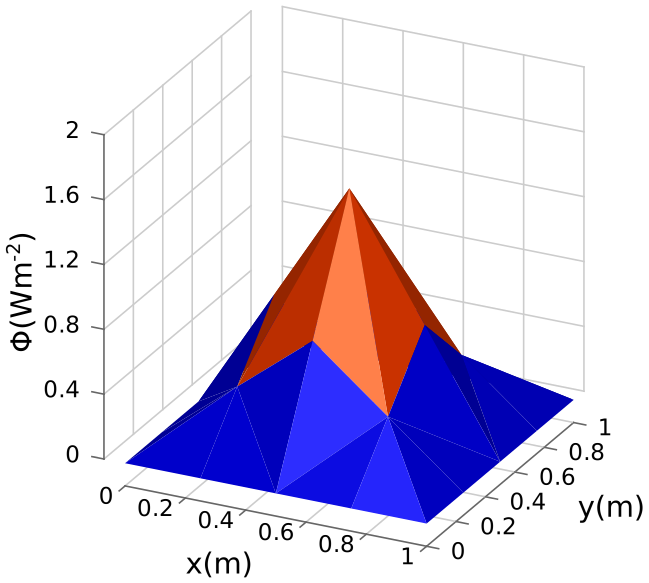
\includegraphics[width=0.49\textwidth]{diagram1}
		\label{fig:diagram1}
	} \\
	\subfloat[Functions]{
		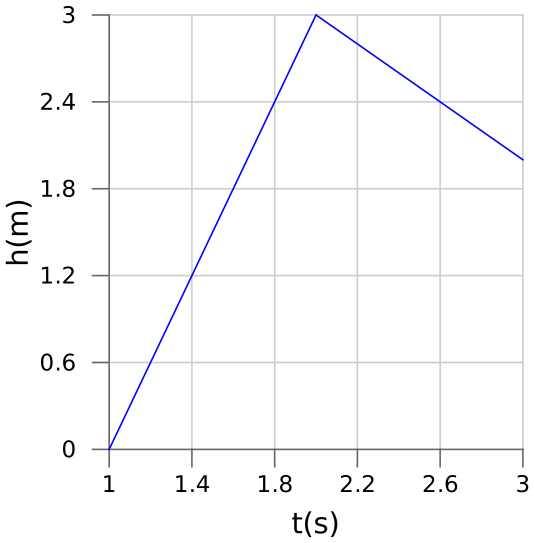
\includegraphics[width=0.4\textwidth]{diagram2}
		\label{fig:diagram2}
	} \hspace{0.5em}
	\subfloat[2D vector field]{
		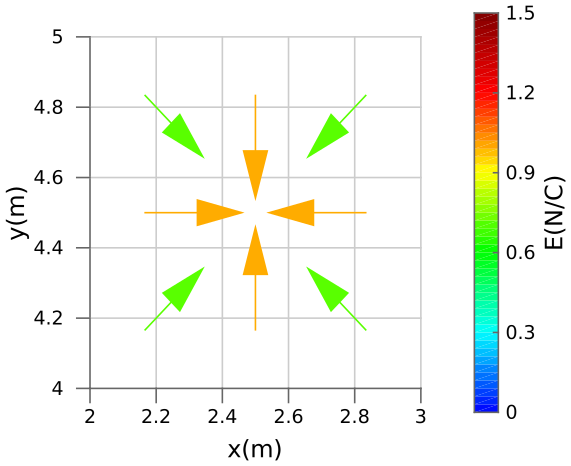
\includegraphics[width=0.52\textwidth]{diagram3}
		\label{fig:diagram3}
	}
	\caption{Data types supported by the program}
	\label{fig:diagram}
\end{figure}

There are three types of data currently supported by this program, which is the same as types given in the example in listing \ref{code:plugin}. The rendering results are given in figure \ref{fig:diagram}. Each type of data uses different generators to convert to models. But all the models follow the same interface. The interface is designed to provide best performance when using OpenGL to render, so all the data is stored in vertex based containers. For each model, it need to provide a list of points. In addition, since the rendering uses flat colouring, each element (line or triangle) will be bound to one point, so each point will also be used to store data for the element. For triangles, it requires colour, normal vector and position (center of three points), which will be used later to generate shader effects. For lines, it only requires colour, so normal vector and position can be left uninitialized.

Another important feature of the model interface is indexed rendering. Figure \ref{fig:index} shows the difference between indexed rendering and non-indexed rendering. To render a rectangle, two triangles are required. In non-indexed rendering shown in figure \ref{fig:index2}, 6 points are required and $\triangle123$, $\triangle456$ will be rendered because point cannot be shared by rectangles. For indexed rendering shown in figure \ref{fig:index2}, 4 points are required and $\triangle123$, $\triangle234$ will be rendered. Since points can be shared in indexed rendering, amount of points can be significantly reduced, which could be especially useful in the current design, where many attributes are bound to points. In flat colouring, points can be ideally reduced to $1/3$, hence reduce memory usage and performance cost in model generation.

Indexed rendering also improves flexibility of the rendering system. For axis and grid, using a interface similar to model interface, some of the points is required to have different position at different view angle. For models, triangles might be sorted in a different order at different view angle. In these scenarios, the developer only need to generate all the points despite the view angle, then use different indexes to select and sort elements according to requirements, which helps to reduce frequency of model regeneration and simplify the logic.

\begin{figure}[!tb]
	\centering
	\subfloat[Indexed rendering]{
		\includegraphics[width=0.2\textwidth]{index1}
		\label{fig:index1}
	} \hspace{2em}
	\subfloat[Non-indexed rendering]{
		\includegraphics[width=0.26\textwidth]{index2}
		\label{fig:index2}
	}
	\caption{Demonstration of indexed rendering}
	\label{fig:index}
\end{figure}

Based on the indexed rendering system, every model provides two core elements: points and indexes. In flat colouring, each elements will be bounded to one point, so the point also needs to store the data for that element. For points, it contains the position of the point, in addition to colour, position and normal vector of the element the point is bound to. The standard implementation requires all the points located in the cube: $x, y, z \in [0, 1]$, which is also the targeted space of axis and grids. For indexes, lists for line index and triangle index are separated because they are the only two element types currently supported in this program.

\subsubsection{Rendering Implementation}

\begin{figure}[!tb]
	\centering
	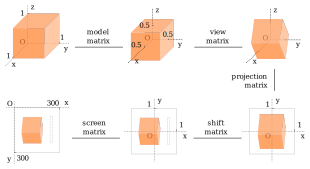
\includegraphics[width=0.95\textwidth]{matrix}
	\caption{Demonstration of transformations in model rendering}
	\label{fig:matrix}
\end{figure}

The core part to render model to desired position is transform matrices. The procedure is given in figure \ref{fig:matrix}. The procedure starts at local space, which is the $1\times1\times1$ cube described in section \ref{sec:model}. After transformation of model matrix, the model will be moved into world space, and the center of the model will be moved to the origin of world space. In world space, shader effects like diffuse and specular lighting will be calculated. Afterwards, the model will be further transformed by view matrix, which enables rotation of the view point. With help of projection matrix, all the shapes will projected into 2D plane, which is know as the screen plane. According to OpenGL specifications, the rendered area is the square $x, y \in [-1, 1]$, so the projection matrix need to be tweaked to the proper scale to make sure the model is included in the square.

The typical implementation for OpenGL rendering stops at projection. But in this project, further transformation may be applied. When colour bar is enabled, the rendered model will be shrank and moved to provide space for the colour bar. This procedure will use a shift matrix to transform. The OpenGL implementation usually stops at shift matrix, but the Qt painting implementation, a different coordinate system is used. The last picture in figure \ref{fig:matrix} shows the range of a widget that is $300\times300$ in pixel. The axis have different direction and the boundary is also changed. Therefore, a screen matrix is used to move all the element from rendering area of OpenGL to the coordinate system of the widget.

Another important difference between OpenGL implement and Qt painting implementation is OpenGL supports depth buffer while Qt does not. For Qt painting system, elements rendered later will be on the top of the picture, which is the typical implementation for 2D painting systems. When rendering a 3D model, this means the triangles need to be sorted in correct order to make sure shapes closer to the camera is rendered later. The render engine do not provide implementation for the sorting algorithm. Instead the sorting process is done by the models with dedicated algorithm for different types of models. When rendering the model, render engine will pass the view angle to the model, then the model will sort the triangles and return to the engine as the order of indexes. The sorting algorithm can be significantly simplified in this way.

\begin{figure}[!htb]
	\centering
	
\includegraphics[width=0.22\textwidth]{dir}
	\caption{Typical view direction}
	\label{fig:dir}
\end{figure}

The widely used algorithm to sort shapes in this project uses a view angle based implementation. 2D data accepted by this program are usually formed as matrices, so they will be rendered as grids. Figure \ref{fig:dir} shows a $3\times3$ grid. The plane is separated to 8 sections, with each section having a \SI{45}{\degree} difference in polar coordinate. Numbers are given to each section as represent in program, then the rendering sequence can be determined according to view direction. The number on each block shows the sequence of rendering when the view direction is within section 0. When rendered in this sequence, farther blocks will always be covered by newly rendered blocks.

\subsubsection{Data Sampling} \label{sec:sampling}

\begin{figure}[!tb]
	\centering
	\subfloat[Point offset]{
		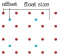
\includegraphics[width=0.25\textwidth]{sample1}
		\label{fig:sample1}
	} \hspace{1.5em}
	\subfloat[Original grid]{
		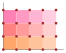
\includegraphics[width=0.28\textwidth]{sample2}
		\label{fig:sample2}
	} \hspace{1em}
	\subfloat[Sampled grid]{
		
\includegraphics[width=0.28\textwidth]{sample3}
		\label{fig:sample3}
	}
	\caption{Demonstration of data sampling}
	\label{fig:sample}
\end{figure}

When rendering a set of data, time cost to generate and render model can be significantly affected by the amount of data points. For normal computers, they should be able to render a $200\times200$ data set without causing noticeable time delay. But for larger data samples, the computer might fail to render the diagram in real time due to performance issues. In addition, for diagram types like vector plot given in figure \ref{fig:diagram3}, each data point will be converted to one arrow. For large data sets, there might be too many arrows to be clearly rendered. Therefore, data sampling is used to reduce the size of grid without causing severe lost of data quality. The implementation can be found in \lstinline{util.h} and \lstinline{util.cpp} \footnote{Available online at \url{https://github.com/PlamaDev/Plama/blob/master/app/util/util.h} and \url{https://github.com/PlamaDev/Plama/blob/master/app/util/util.cpp}.}. Although the implementation is not part of rendering module, it is described within the rendering module since it is widely used in the module.

Figure \ref{fig:sample} shows the logic with sampling ratio of 2, which means every $2\times2$ grid will be sampled into one point. The original grid is a $5\times4$ gird, shown in red points. After sampling the data is converted to a $2\times2$ grid, shown in blue points. In the current implementation, average of numbers is calculated as the sampled value because it keeps linearity and will include all the data.

During the sampling procedure, several attributes will be generated:

\begin{itemize}
	\item \textbf{Offset:} As is shown in figure \ref{fig:sample1}, the sampling procedure will generate an offset between original grid and sampled grid. This will lead to the empty boundary when rendering the sampled grid.
	\item \textbf{Original size:} The sampler will record the original size of data. The variable name in program is \lstinline{s_o}.
	\item \textbf{Integer size:} For the given data sample, only two columns of data will be generated and the last column will be ignored because it can not form a complete $2\times2$ gird. So the integer size will be 2 in horizontal direction. The variable name in program is \lstinline{s_i}.
	\item \textbf{Float size:} Although the last column cannot be sampled, the space should be left empty. Float size is used to describe the expected space consumption of the sampled grid. In the example, it should take the width of 1.5 blocks (with last half block left empty) in horizontal direction, so the float size is 1.5. The variable name in problem is \lstinline{s_f}.
\end{itemize}

When generating models, data sampler will be used as the wrapper of raw data, which will automatically provide sampled data to accessors, which provides consistence and convenience when accessing data with sampling enabled. When generating models, implementations should fully consider the effect of data sampling and make full use of attributes generated to ensure the shapes are placed at desired location.

\subsubsection{Model Generation}

\paragraph{Surface Model}

\begin{figure}[!tb]
	\centering
	\subfloat[Top view]{
		\includegraphics[width=0.38\textwidth]{unit1}
		\label{fig:unit1}
	} \hspace{1.5em}
	\subfloat[3D view]{
		\includegraphics[width=0.38\textwidth]{unit2}
		\label{fig:unit2}
	}
	\caption{Demonstration of block separation}
	\label{fig:unit}
\end{figure}

This model aims to convert two dimensional scalar data into height in a surface like the diagram in figure \ref{fig:diagram1}. When generating the model, data will be separated into blocks each containing 4 data points, as minimum units. A generating algorithm is implemented to convert one block into a small section of the surface. By repeating the generating algorithm to each block, sections will be combined into a surface. Figure \ref{fig:unit} shows the method to render one block. Each block is separated into 8 triangles. The typical implementation for programs like \MatLab{} and Octave uses the separation shown in figure \ref{fig:index}, where each block is separated into two triangles and the colour is usually decided by one of the point, which explains the asymmetry of the rendering result in figure \ref{fig:matlab1} and \ref{fig:matlab2}. Compared to their implementation, the advantage of this method is that the separation is symmetrical, and data from all 4 points will be included in the block because the colour of each triangle is decided by the closest point. The disadvantage is it creates about 4 times of triangles compared to the implementation of \MatLab{} and Octave. However, the performance lost related to amount of triangles can be compensated by OpenGL rendering and other performance optimizations. The implementation is given in function \lstinline{genHeight} in \lstinline{render/model.cpp}\footnote{\label{ftnt:model}Available online at \url{https://github.com/PlamaDev/Plama/blob/master/app/render/model.cpp}}.

\paragraph{Vector Model}

\begin{figure}[!tb]
	\centering
	\subfloat[Original grid]{
		\includegraphics[width=0.383\textwidth]{vec1}
		\label{fig:vec1}
	} \hspace{1.5em}
	\subfloat[Grid sampled with factor 2]{
		\includegraphics[width=0.4\textwidth]{vec2}
		\label{fig:vec2}
	}
	\caption{Demonstration of point positioning}
	\label{fig:vec}
\end{figure}

Vector model aims to convert data of a vector field to arrows in the space. The generation of the model is relatively easy compared to that of surface model. An algorithm is implemented to convert one data point to an arrow in the figure. Repeating the same process to each data point, the figure can be completed. The implementation mainly consists of a number of conversion between Cartesian coordinate and polar coordinate, to move and scale the arrow, but the most difficult part is calculating the offset. Figure \ref{fig:vec} shows elements affecting the location of roots of arrows:

\begin{itemize}
	\item \textbf{Margin:} The margin is set to be half the size of a block without sampling. It is used to make space for arrows on the boundary, and also to keep consistence with MD2D model described in section \ref{sec:md2d}. It is usually called \lstinline{margin_} in the code.
	\item \textbf{Grid difference:} The distance between two adjacent lines in the grid, which might be increased by data sampling. It is usually called \lstinline{diff_} in the code.
	\item \textbf{Sampling offset:} As is described in section \ref{sec:sampling}, data sampling will generate an offset to the grid. It is usually called \lstinline{offset_} in the code.
\end{itemize}

The implement for vector model generation is given in function \lstinline{genVector} in file \lstinline{render/model.cpp}\footnotemark[\getrefnumber{ftnt:model}].

\subsection{GUI Module}

The main purpose of GUI module is to provide the interface to interact with the user. The implementation of the main window can be found in \lstinline{gui/windowmain.h} and \lstinline{gui/windowmain.cpp} \footnote{Available online at \url{https://github.com/PlamaDev/Plama/blob/master/app/gui/windowmain.h} and \url{https://github.com/PlamaDev/Plama/blob/master/app/gui/windowmain.cpp}.}. Since development of the interface is typical for Qt widget applications and it is mainly invoking APIs provided by other modules, the implementation will not be introduced in detail.

As an important part of the GUI module, Plot widget is developed as place holder of diagrams. As a subclass of \lstinline{QWidget}, it aims to provide clear interface to developers including setting the quantity, time, rotation and sampling factor. As the controller of rendering medium, it also handles setup operations when exporting to images and provides implementation to export the quantity into video. Generally speaking, it functions as the simplified collection of APIs provided by rendering module, and the controller of one figure.

\subsubsection{Rendering Medium Selection} \label{sec:medium}

It might be confusing to some people that the selection of rendering medium can have significant effect to performance and quality, but the difference can be easy to notice especially in native development. Here lists some rendering media available:

\begin{itemize}
	\item \textbf{QWidget:} \lstinline{QWidget} is a very important element in Qt framework. For image rendering, it provides unified interface to native implement, usually based on the raster engine running on CPU. The disadvantage is the behaviour can be widely affected by the native implementation. An example is text rendering. On Windows, ClearType (font antialiasing) will only be enabled for font larger than 18, making the rendering of small texts look ugly. In addition, the algorithm for ClearType is not suitable for rotated text, making vertical text looks wired. The performance is also not good enough for heavy rendering loads. The rendering of diagrams was once implemented using native rendering but performance lost was painful.
	\item \textbf{QOpenGLWidget:} The widget \lstinline{QOpenGLWidget} is the method suggested by Qt for OpenGL based rendering. It is easy to use with OpenGL because it provides separate entry for initialization and rendering phase, which is required in typical implementation for OpenGL rendering. However, the official implementation of this widget seems not optimized or have bug in the latest version. When using this widget in a window, the window might become slow for resizing operations. After some configurations, the performance seems acceptable, but delay can still be noticed.
	\item \textbf{QWindow:} As is indicated by the name, class \lstinline{QWindow} creates a window. This class provides low-level implementation for interface rendering, which means many features like automatic frame swapping can be disabled to provide best performance. Another benefit of \lstinline{QWindow} is a window rather than widget, so it will not affect the behaviour of other widgets in the same window. When used, calling \lstinline{QWidget::createWindowContainer} can easily convert it into a widget to be place into the interface. The disadvantage is that it lacks some important features like mouse dragging, so the required features in addition with OpenGL context setup is required to be implemented manually.
	\item \textbf{QImage:} Class \lstinline{QImage} is the rendering medium stored in memory. So it can be used for off-screen rendering, which could be helpful when exporting images. Another advantage is that it is less platform dependent compared to on-screen implementations, so the texts usually have better quality compared to native implementation on Windows. The disadvantage is the performance is not good enough for real time rendering. When using \lstinline{QImage} as buffer for on-screen rendering, the content need to be rendered to the image, then the entire image is required to be rendered to window, which could cost more performance than usual. So the developer need to be very careful with the usage of images.
	\item \textbf{QSvgGenerator:} Class \lstinline{QSvgGenerator} is another rendering medium provided by Qt in SVG module. Different from all the media described previously, \lstinline{QSvgGenerator} uses vector image engine rather than raster engine. Therefore, vector images can be easily generated. This medium is not compatible with OpenGL, which means all the rendering (including 3D rendering) is required to be processed as 2D shapes.
	\item \textbf{QOpenGLWindow:} Class \lstinline{QOpenGLWindow} is said to be the alternate for \lstinline{QWindow} with optimizations for OpenGL, but it not test due to limited time.
\end{itemize}

After the investigation, for on-screen rendering, the implementation uses \lstinline{QWindow} as the base. All the texts are rendered into one image, then moved to the \lstinline{QWindow}. Other elements will be rendered directly into \lstinline{QWindow} using OpenGL. For figure export, \lstinline{QImage} and \lstinline{QSvgGenerator} will be used for raster and vector images because they usually provide better quality.

\subsubsection{Video Exporting}

This program uses FFmpeg to generate video. Firstly, all the frames will be rendered into images and stored in temporary directory provided by \lstinline{QTemporaryDir}. Afterwards, FFmpeg will be invoked as external process because it provides simpler interface and it easier to maintain. When generating frames, image will be saved in lossless mode, then compressed during video encoding, which can provide descent video quality with small file size.

\section{Result}

\subsection{User Interface}

\begin{figure}[!tb]
	\centering
	\includegraphics[width=\textwidth]{interface}
	\caption{Screen capture of user interface}
	\label{fig:interface}
\end{figure}

The screen capture of the program is given in figure \ref{fig:interface}. On the left hand side, a tree structure is used to describe the project structure described in section \ref{sec:datastruct}. On the top, a slider is used to help the user select the time. By dragging the slider, all the plots will be updated automatically, which enables the user to view all the quantities easily at a certain time. For each figure, a toolbar is given with buttons to export the diagram and toggle all the features like shader effect, colour bar and data sampling individually for each diagram.

All the components in the window except the slider bar is implemented as \lstinline{QDockWidget}, which supports resizing and reorganizing. The user can easily modify the layout of the interface by drag and drop. Diagrams can be even dragged out of the window as floating window, which makes the layout more flexible.

\subsection{Compilation and Distribution}

This project is hosted on Github and all the source code is available in the online repository \footnote{Link: \url{https://github.com/PlamaDev/Plama}.} with a short documentation. For Linux users, they can clone the repository to local directory and compile by themselves. For Windows users, they can use the executable file given in release page \footnote{Link: \url{https://github.com/PlamaDev/Plama/releases}.}.

This project uses qmake provided by Qt as the compiling environment. To compile the project on Linux, package \lstinline{qt5-base}, \lstinline{qt5-svg}, \lstinline{ffmpeg} and \lstinline{python}(over python 3) should be installed and linked. On Arch Linux, the packages can be installed by executing \lstinline{sudo pacman -S qt5-base qt5-svg python ffmpeg}. The command should be similar on other Linux distributions. Afterwards, by executing \lstinline{sudo qmake && make && make install}, the program will be compiled and installed.

For Windows users, compiling the code is not suggested because configuring the development environment and gathering library files might be difficult and time consuming. The executable file is compiled in Qt Creator using MinGW. The executable file cannot be distributed directly because it cannot find dlls (dynamically linked libraries) required. There are two ways to help the program link to libraries: including the library file in system path or put the files in the same directory. The latter one is usually chosen because it provides convenience for distribution. Finally, to make the program portable, all the files including the executable and libraries are compressed into a self-extracting file. When the program is executed, it will automatically extract all the files into a system temporary directory, then execute the original program. Using this method, the program can be distributed as one file, which significantly improves convenience in distribution. However, the disadvantage is the entire program will be extracted every time it executes, so it might take about 2 extra seconds when starting.

\subsection{Output Quality}

\begin{figure}[!tbp]
	\centering
	\subfloat[JPG output by this program]{
		\includegraphics[width=0.47\textwidth]{comp1}
		\label{fig:comp1}
	} \hspace{0.5em}
	\subfloat[PDF output by this program]{
		\includegraphics[width=0.47\textwidth]{comp2}
		\label{fig:comp2}
	} \\
	\subfloat[JPG output by Octave]{
		\includegraphics[width=0.47\textwidth]{comp3}
		\label{fig:comp3}
	} \hspace{0.5em}
	\subfloat[PDF output by Octave]{
		\includegraphics[width=0.47\textwidth]{comp4}
		\label{fig:comp4}
	} \\
	\subfloat[JPG output by \MatLab{}]{
		\includegraphics[width=0.47\textwidth]{comp5}
		\label{fig:comp5}
	} \hspace{0.5em}
	\subfloat[PDF output by \MatLab{}]{
		\includegraphics[width=0.47\textwidth]{comp6}
		\label{fig:comp6}
	}
	\caption{Comparison of rendering outputs for equation \ref{eq:surf}}
	\label{fig:comp}
\end{figure}

\begin{lstfloat}[!tb]
	\begin{lstlisting}[language = python, style = mybase, label = code:surf,
	caption = Plugin to generate the surface]
from math import exp

def gen():
	ret = []
	for yi in range(20):
		for xi in range(20):
			x = -2 + 2 / 19 * xi
			y = 2 / 19 * yi
			ret.append(2 / exp((x-0.5)**2 + y**2) - 
				2 / exp((x+0.5)**2 + y**2))
	return ret

class Loader:
	@staticmethod
	def name():
		return 'Test'

	@staticmethod
	def load():
		return [{
			'abbr': 'Test',
			'name': 'Test',
			'children': [],
			'quantities': [{
				'name': 'Surface',
				'times': [1],
				'dimData': 1,
				'sizeData': [20, 20],
				'sizeModel': [[-2, 0], [0, 2]],
				'labels': ['', '', '', ''],
				'data': lambda: [
					gen()
				]
			}]
		}]

	@staticmethod
	def args():
		return []

plugin = Loader()
\end{lstlisting}
\end{lstfloat}

This program support several image formats: JPG, PNG, SVG and PDF. For PNG images, they have transparent background. For SVG and PDF, the image is generated completely by vector elements. For video export, the quality is good enough and output file is well compressed, but the video encoding might be further tweaked for compatibility with old players.

Figure \ref{fig:comp} shows output files generated by this program, in addition with diagrams generated by Octave and \MatLab{} for surface given in equation \ref{eq:surf} with $x\in[-2, 0]$, $y \in [0, 2]$. Since the gradient currently cannot be configured in this program and flat lighting is the only supported lighting method, other programs are configured to similar settings.

\begin{equation} \label{eq:surf}
	z = \frac{2}{e^{(x - 0.5)^2 + y^2}} - \frac{2}{e^{(x + 0.5)^2 + y^2}}
\end{equation}

To help the program render the surface, a plugin is written to generate the data on the surface. The code of the plugin is given in listing \ref{code:surf}. This can also be the used as demonstration of plugins used for function and surface rendering, which also shows the flexibility of the plugin system.

In the comparison, since light reflection in this program is more conservative and the surface is divided into more triangles, the lighting is slightly different. For JPG export, file generated by Octave is not well antialiased and file generated by \MatLab{} seems over-compressed (using default settings), causing slightly distortion at the edges. For PDF export, Octave cuts the surface into too many triangles, possibly because the vector image is regenerated from raster rendering. For \MatLab{}, the rendering quality is good and some of the triangles are even reduced to reduce file size. Generally speaking, the render quality of this program can be considered competitive compared with professional software. The rendering of surface and axis are good in both raster and vector image, but range of axis and distribution of the gradient can still be optimized.

\section{Discussion}

\subsection{Difficulties in Development}

There are several special issues in the development of this project. The first is the scale of numbers. Integer types, especially \lstinline{short} are usually considered to be easy to overflow in daily development, but overflow of float types are relatively uncommon. However, since the data used in this project are usually generated in simulation, the numbers can be incredibly large, sometimes close to the maximum limit of float numbers. For numbers at this scale, extra attention should be given because any mathematical operations could easily cause overflow. Taking Pythagorean theorem as an example. The typical form given in equation \ref{eq:pt1} will double the scale of numbers in calculation, causing risks of overflow. Instead, the form given in equation \ref{eq:pt2} is used with $k=max(a, b)$, which can be helpful to prevent float overflow. In addition, most of data types used in this program is moved from \lstinline{float} to \lstinline{double}, which could improve the reliability.

\begin{align}
	c &= \sqrt{a^2 + b^2} \label{eq:pt1}\\
	c &= k\sqrt{(\frac{a}{k})^2 + (\frac{a}{k})^2} \label{eq:pt2}
\end{align}

Another problem is compiling and distribution on Windows. Visual Studio is widely used for development on Windows, but the configuration uses a heavy system provided by microsoft, which is difficult to maintain and can easily break consistence with the code base on Linux, as the main reason to switch the compiler from Visual Studio to MinGW. Another problem is some new features of C++ is not fully supported. To use new features like initialization list and function \lstinline{make_unique}, extra configurations are required. Linking the library files also takes a long time to be configured correctly because the developer is not so familiar with native development on Windows.

Compatibility issues are also painful. As is introduced in section \ref{sec:render} and \ref{sec:medium}, many approaches has been tried and many of them has been abandoned, which is the main reason to slow down the development speed, especially in early stages. Documentations are also difficult to find about these topics, possibly because there are not so many projects with performance pressure like this project. The main method to solve these problems is to try different approaches manually. However, the implementation for different approach might be so different, making many code written, but deleted. The current choice seems reasonable in both performance and compatibility, except for some delay when resizing the window on Windows. So the choices can be further improved.

\subsection{Review of Code Quality}

The current code base has about 3300 lines, containing code written in C++, Python and GLSL. The main aim of coding is to keep the project easy to maintain. Therefore, features are separated into modules and classes for decoupling. A typical example is rendering module. Each element in the figure including model, axis and colour bar has been separated to an object-oriented structure, so that the implementation of each element can be easily found and modified without affect other elements. The code base has been refactored several times, reduced from peak amount of more than 5000 lines. During the refectories, many redundant and deprecated code was removed, making the code short can clean. Self-explanatory is also one of indicators of good code quality \cite{ref:cleancode}. The structure and implementation of code seems to be clear enough for beginners to understand, except for some important functions having significant effect to performance, where some low level optimizations and advance design patterns are used, making the code slightly more difficult to understand.

There are also many aspects to be improved. The code is lacking documentation and comments can only be found in long functions or variable name abbreviations. Although the code is not difficult to maintain for developers understanding the structure of project, it could still lead to the impression that the project is lacking maintenance. Another problem in the project is APIs in this project are not fully split. For developers intending to use this project as rendering library, it might not be easy to configure.

\subsection{Future Suggestions}

Although the current implementation seems to be reasonable for testing purpose, there are still many details to be improved and many features to be added:

\begin{itemize}
	\item The export files have hard-coded file size. It can be helpful if the user can adjust the configurations.
	\item In the plugin protocol, only the data uses lazy loading, but for some file encodings, other attributes like time list cannot be generated without analysing the entire file. It could be helpful to make more attributes use lazy loaded.
	\item In this project, models will be generated in real time when the data change, which requires a very fast implementation in model generation. The current solution seems acceptable, but it might be significantly improved if the calculations is processed in GPU because profiling results indicate the most time consuming part is vector operations like cross product and normalization, which are strengths of GPU.
	\item As an important feature, decorators are widely used in modern Python frameworks. The main benefit of it is that it provides simplicity in member registering and event handling. Typically it can help remove more than 10 lines of redundant code and class structure, making the structure more light weighted. The disadvantage is it requires one extra python dependency, making it not so straightforward for beginners. Therefore, the design is still being considered.
	\item The current implementation use HTML notations for rich text formatting because it is supported by Qt. However, for academic users, they might be more familiar with format notations in \LaTeX{} format, which is also the choice in \MatLab{} and Qucs\cite{ref:qucs} (a circuit simulator). It is not currently implemented because the implementation requires good understanding of both HTML and \LaTeX{}, and might require take much effort.
	\item In current implementation, libraries use different methods to load. On Linux, shared libraries are used. On Windows, the executable is distributed with all the dependencies. In this case, Python packages installed to the system will also be available to plugins on Linux, but will have no effect on Windows because the embedded libraries will always be linked no matter if Python is install on Windows. The path of Python library should be configurable, making it possible for plugins to use Python packages installed to the system.
	\item The plugin protocol uses relatively a static structure. Once the data is loaded, they will be stored in memory and should not be modified. However, the protocol can be expanded to accept data stream or other dynamic data sources by adding the refreshing options, which could make the program applicable to more scenarios.
\end{itemize} 

\section{Conclusion}

The development of this project has been generally completed. In this project, a program to view plasma simulation files is developed. In addition, the frameworks is expanded to be flexible enough to accept many types of data from different sources. During the development process, although most of the time is used to test and solve compatibility issues, there are many exciting moments when high quality implementations are made, and when difficult problems are solved. When faced with design choices, the method with more potential is usually chosen. When rendering the data, an entire rendering system is implemented when there are already several mature solutions. Although the system is not so rich in feature compared to other solutions, test results indicate it has outstanding performance and descent rendering quality in default settings, so it might be the most suitable solution in this project. There are several implementation details like rendering of axis and positioning of axis labels not introduced in this report because they are not so important regarding to the general quality of the program. However, the optimizations in the details can be reflected in the user experience. There are still many details to be improved and even several bugs to be fixed. Following improvement suggestions provided in previous sections, the project can also be further improved to be applicable for other fields.

\bibliographystyle{res/myieee}
\bibliography{reference}
\addcontentsline{toc}{section}{References}

\clearpage
\begin{appendices}

\section{Project Specification}

Here is the quote of the original project specification, which have not been modified:

\begin{quote}
	Microplasmas are electrical discharges with dimensions less than 1 mm, and have a range of application from plasma televisions to biomedicine. The Technological Plasma Group has an existing simulation code for microplasmas that generates large amounts of output data in various formats. The aim of this project is to develop a user-friendly interface that effectively displays the simulation output. An initial phase of the project will involve familiarisation with running the simulation code. The main part of the project will involve using C++ to develop a standard ``dashboard'' for the simulation that allows the user to view static graphs and videos of the simulation output in a format that is intuitive and simple-to-use. The design of such an interface is a key aspect of enabling sophisticated simulation software to being widely accessible to industry users.
\end{quote}

Figure \ref{fig:gantt} shows the Gantt chart given in preliminary report. During the development, progress generally follows the plan, but took more time on rendering library, less time on exporting library.

\begin{figure}[!htb]
	\centering
	\includegraphics[width=0.9\textwidth]{gantt}
	\caption{Gantt chart in preliminary report}
	\label{fig:gantt}
\end{figure}

\end{appendices}

\end{document}
